\documentclass{article}
\usepackage[utf8]{inputenc}
\usepackage{graphicx}

\title{Misura di h con fotocellula}
\author{Francesco Pio Merafina, Onofrio Davide Caputo, Alessandro Lamesta}
\date{}

\begin{document}
\maketitle
\section{Abstract:}
L'idea è quella di utilizzare una fotocellula in cesio per poter calcolare la costante di Planck e la funzione lavoro della fotocellula usando diversi tipi di luci.
~
\section{Cenni teorici:}
Sappiamo che un fenomeno di interazione radiazione e.m. e materia è l'effetto fotoelettrico, mediante il quale possiamo esstrare elettroni da un atomo usando la giusta energia. Infatti sappiamo che l'energia cinetica con la quale uscirà l'elettrone sarà la differenza tra l'energia del fotone ed una funzione che rappresenta il lavoro necessario per poter estrarre l'elettrone; questa funzione è chiamata funzione lavoro o work function.
~
\section{Apparato sperimentale:}
L'apparato sperimentale consiste in un apparecchio contenente una fotocellula al cesio, un alimentatore per led, un voltmetro, un amperometro, un potenziometro, ed un dispositivo per la variazione della luce. I led sono rispettivamente:
\begin{itemize}
    \item blu = 472nm
    \item verde1 = 505nm
    \item verde2 = 525nm
    \item giallo = 588nm
    \item rosso = 611 nm
\end{itemize}
~
\section{Metodologia di misura:}
La metodologia di misura è stata analoga per tutti e 5 i led. Si è inserito il led nell'apposito alloggiamento, avendo cura di non esporre la fotocellula alla luce della stanza, si sono settati 3 valori di intensità della luce del led (25$\%$, 50$\%$, 75$\%$) e si è fatto variare il potenziometro. La variazione del potenziometro è stata eseguita mediante due manopole, una più "fine" ed una più "grezza"; usando il potenziometro si sono selezionati dei valori di d.d.p. ed usando l'amperometro si sono segnati i valori di corrente, fino a quando non si osservava più corrente.
~
\section{Analisi dati:}
Osservando i grafici ottenuti però non sono corretti in quanto si può osservare la di correnti negative in presenza di potenziali di arresto positivi, il che ci fa pensare che in verità i dati riportati dallo strumento hanno i segni invertiti. Quindi correggendo i grafici otteniamo i risultati corretti; una nota importante va fatta per le incertezze, la quale è stata associata al potenziale di arresto, definito come punto del piano I-V tale che I=0, l'incertezza è stata associata come la differenza tra la tensione che restituisce I=0 e la tensione tale che I=±0.002A . In questa maniera possiamo osservare quali sono i potenziali di arresto per i singoli led. Per verificare una effettiva dipendenza di carattere lineare tra potenziale di arresto e funzione lavoro, si sono fatti dei plot su un piano frequenza-tensione. Le formule di riferimento sono:
Effetto fotoelettrico:
\begin{equation}
    K_{e^{-}}=h\nu-W_{0}
\end{equation}
Che nel caso particolare in cui l'energia cinetica dell'e$^{-}$ sia uguale al potenziale di stop otteniamo una relazione lineare:
\begin{equation}
    V_{0}=\frac{h\nu}{e}-\frac{W_{0}}{e}
\end{equation}
Quindi la pendenza della retta di fit dei potenziali di stop a diverse frequenze, moltiplicata per la carica dell'elettrone restituisce la costante di Planck, analogamente per l'intercetta da cui otteniamo la funzione lavoro.
Avendo usato tre diversi valori di intensità della luce, per ottenere h e W$_{0}$ usiamo una media pesata:
\begin{equation}
    h=\frac{\sum\frac{h_{i}}{\sigma_{i}^2}}{\sum\frac{1}{\sigma_{i}^2}}
\end{equation}
\begin{equation}
    W_{0}=\frac{\sum\frac{W_{0i}}{\sigma_{i}^2}}{\sum\frac{1}{\sigma_{i}^2}}
\end{equation}
~
\section{Risultati e conclusioni:}
Quindi prendendo i dati dai grafici corrispondenti alle figure 1,2 e 3 otteniamo h=(6.34$\pm$0.29)10$^{-34}$Js, compatibile entro una sigma con il valore vero, passando alla funzione lavoro, essa vale W$_{0}$=1.85$\pm$0.10 eV, la quale è vicina, ma non compatibile con il valore vero della funzione lavoro del cesio che risulta essere 2.14eV; ciò potrebbe essere attribuibile ad eventuali perdite dovute ad una eventuale non corretta illuminazione della fotocellula, e quindi perdita di fotoni incidenti.
~
\section{Tabelle e grafici}
\begin{figure}[h!]
    \centering
    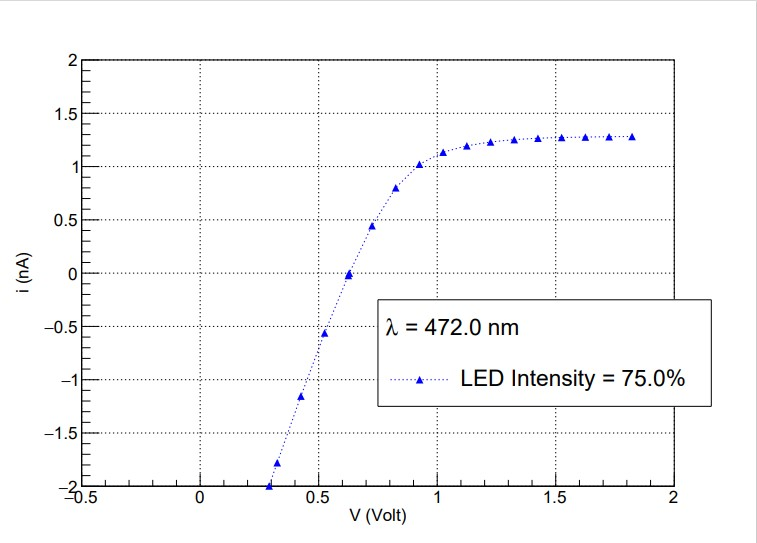
\includegraphics[width=\linewidth]{blu75.jpg}
    \caption{Andammento I-V della fotocellula con luce blu incidente al 75$\%$ di intensità}
    \label{figura1}
\end{figure}
\begin{figure}[h!]
    \centering
    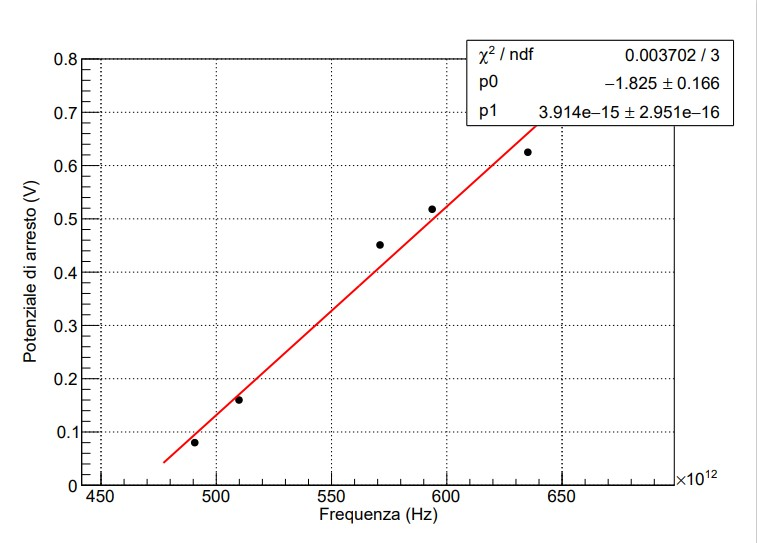
\includegraphics[width=\linewidth]{plot25.jpg}
    \caption{Plot dei potenziali di arresto al 25$\%$}
    \label{figura1}
\end{figure}
\begin{figure}[h!]
    \centering
    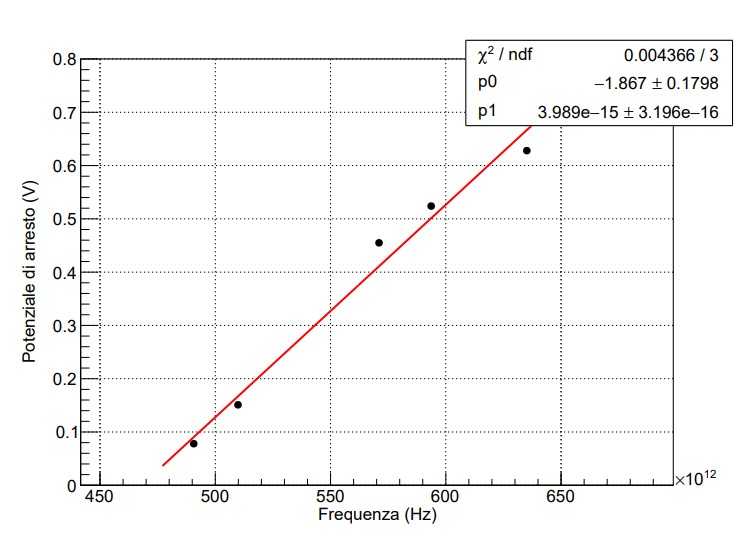
\includegraphics[width=\linewidth]{plot50.jpg}
    \caption{Plot dei potenziali di arresto al 50$\%$}
    \label{figura1}
\end{figure}
\begin{figure}[h!]
    \centering
    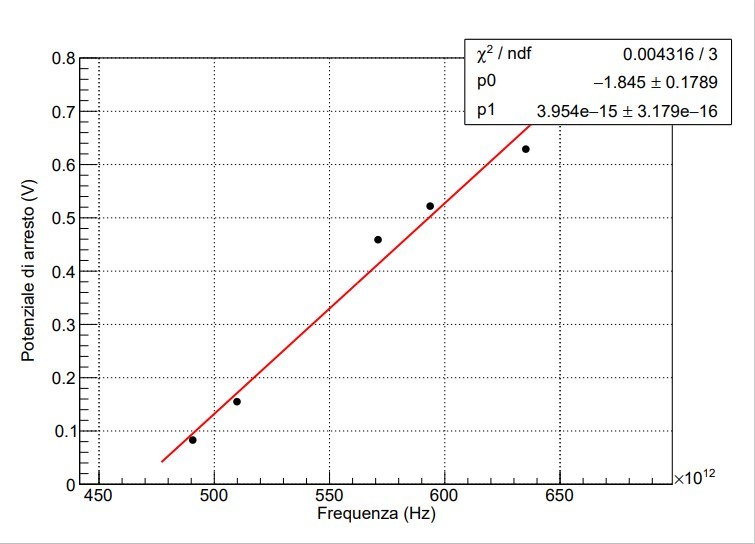
\includegraphics[width=\linewidth]{plot75.jpg}
    \caption{Plot dei potenziali di arresto al 75$\%$}
    \label{figura1}
\end{figure}
\begin{table}[h!]
  \begin{center}
   \begin{tabular}{|c|c|c|}
      $\lambda$[nm]&I[$\%$]&V$_{0}$[V]\\
      611&25&0.080$\pm$0.005\\
      588&25&0.160$\pm$0.038\\
      525&25&0.451$\pm$0.001\\
      505&25&0.518$\pm$0.001\\
      472&25&0.625$\pm$0.001\\
      611&50&0.078$\pm$0.007\\
      588&50&0.151$\pm$0.018\\
      525&50&0.455$\pm$0.001\\
      505&50&0.524$\pm$0.001\\
      472&50&0.628$\pm$0.001\\
      611&75&0.083$\pm$0.003\\
      588&75&0.155$\pm$0.013\\
      525&75&0.459$\pm$0.001\\
      505&75&0.522$\pm$0.001\\
      472&75&0.629$\pm$0.001\\
   \end{tabular}
   \caption{Tabella contenente i valori di potenziali di stop, al variare dell'intensità della luce incidente}
  \end{center}
\end{table}
\end{document}